% ======================= Pre-Amble =========================
      
%Format
\documentclass[11pt, oneside]{article}   	% use "amsart" instead of "article" for AMSLaTeX format 
                     						%imports package {article} and specify option(s) [11pt, oneside]
\usepackage{geometry}                		% See geometry.pdf to learn the layout options. There are lots. 
    \geometry{letterpaper}                   		% ... or a4paper or a5paper or ... 
    %\geometry{landscape}                		% Activate for rotated page geometry

\usepackage[parfill]{parskip}    		        % Activate to begin paragraphs with an empty line rather than an indent

    %Colours
    \usepackage{graphicx, subcaption}
    \usepackage[usenames, dvipsnames]{color}     % font colour:    \textcolor{<colour>}{text}
          									%highlight text:  \colorbox{<color>}{text}
    \usepackage{soul}						%highlight text: \hl{}     %only  yellow								
    									%list of colours: https://www.sharelatex.com/learn/Using_colours_in_LaTeX
    									
    %Bullets
    \usepackage{enumerate}     %specify type of enumeration: \being{enumerate}[<type of enumeration>]
    
    %Footnote Spacing
    \setlength{\footnotesep}{0.4cm}                  %specify spacing b/w footnotes
    \setlength{\skip\footins}{0.6cm}                    % space b/w footnotes and textbody


%Mattematics
    %American Mathematics Society packages
    \usepackage{amsmath}	   %math
    \usepackage{amssymb}       %symbols
    \usepackage{amsthm}          %theorems

    %QED
    \newcommand*{\QEDA}{\hfill\ensuremath{\blacksquare}}         %make qed filled square:    \QEDA
    \newcommand*{\QEDB}{\hfill\ensuremath{\square}}               %make qed empty square: \QEDB 
    
    \renewcommand\qedsymbol{\ensuremath{\blacksquare}}		%Proof environment


%Figures
\usepackage{caption}
\captionsetup[figure]{labelfont=bf}    %make figure labels boldface
\captionsetup[table]{labelfont=bf}     %make table labels boldface

\usepackage[hidelinks]{hyperref}                % Allows for clickable references

    %Tables
    \usepackage[none]{hyphenat}                    % Stops breaking-up words in a table (i.e. no hyphens)                                                             
    
    \usepackage{array}   
        \newcolumntype{x}[1]{>{\centering\let\newline\\\arraybackslash\hspace{0pt}}p{#1}}       %center fixed column width: x{<len>}                      
        \newcolumntype{$}{>{\global\let\currentrowstyle\relax}}                                                   % let us apply things (e.g. bold/italicize) to entire row            
        \newcolumntype{^}{>{\currentrowstyle}}
        \newcommand{\rowstyle}[1]{\gdef\currentrowstyle{#1} #1\ignorespaces}
    
    %Images
    \graphicspath{ {images/} }                          %directory that your images are located in within your current directory
    
    %Diagrams
    \usepackage[latin1]{inputenc}
    \usepackage{tikz}
    	\tikzset{line/.style={-latex'}}
        \usepackage{tkz-berge}
        \usetikzlibrary{shapes,arrows}
        \usetikzlibrary{patterns}			%Specify colours of stuff (e.g. vertices): 
        								%	-> set style: \tikzset{VertexStyle/.append style = {minimum size = 8pt, inner sep = 0pt}} 
								%	-> change individual vertices: \AddVertexColor{white}{1,2} 


%Bibliography
\usepackage[numbers,sort&compress]{natbib}   %for multiple references: sorts  (i.e. [1,2] NOT [2, 1] )
                                           				  %                                     compresses (i.e. [1-3] )
\usepackage[nottoc]{tocbibind}                            %add bibliography to table of contents


%Miscellaneous
\usepackage{dirtytalk}    %quotations: use \say  


%================== Header & Footer =========================
\usepackage{fancyhdr}
\usepackage{lastpage}      %ensures you can reference LastPage (i.e. Page 2 of 10)

\renewcommand{\headrulewidth}{0.4pt}		%Decorative Header line: thickness={0.4pt}
\renewcommand{\footrulewidth}{0.4pt}		%Decorative Footer line: thickness={0.4pt}

\setlength{\headheight}{13.6pt} 		%space b/w top of page & header
\setlength{\headsep}{0.3in}		%space b/w page header and body

%Make Header & Footer    
\pagestyle{fancy}
    \lhead{Stephanie Knill} 		% controls the left corner of the header
    \chead{} 					% controls the center of the header
    \rhead{} 					% controls the right corner of the header
    \lfoot{} 					% controls the left corner of the footer
    \cfoot{Page~\thepage\ of \pageref{LastPage}} 				% controls the center of the footer
    												%Page~\thepage\  if just want Page x
    \rfoot{}			 		% controls the right corner of the footer

% =============================== Document ===================================
\begin{document}

% Title Page
\title{MATH 442 --- Assignment 5 \\
\line(1,0){360} \\              %(slope x, y){length of line}
}
\author{
Stephanie Knill \\
54882113 \\
Due: February 4, 2016}

\date{}                   % Activate:  display a given date (e.g. {August 4} ) or no date (empty {} )
                                    %No activate: display current date
\maketitle

%\thispagestyle{empty}                   %Remove header from this (first) page. Change empty -> plain to keep numbering
%								-> Doesn't matter in this case (b/c title page)
%\cleardoublepage


% ================= Questions ================

\section*{Question 25}

\textbf{Proposition:} If a graph has no closed paths of odd length, then it is bipartite.

\textbf{Proof by Contradiction} 

Let there be a graph $G$ that has no closed paths of odd length and is not bipartite. We will denote a closed path of even length by $v_1 \rightarrow v_2 \rightarrow \ldots \rightarrow v_m \rightarrow v_1$.

For a bipartite graph, we can colour all vertices 2 colours, say black and white, such that each edge joins a black and a white vertex. Without loss of generality, we will colour a vertex $v_i$ black if $i=2k+1$ and white if $i=2k$, for some $k \in \mathbb{Z}$. Then we have that $v_1$ is black, $v_2$ is white, $v_3$ is black, ... , and $v_m$ is white. However, $v_m$ and $v_1$ are different colours, so they can be joined by an edge thereby making it bipartite and contradicting our initial assumption. \QEDA


\section*{Question 26}

If a simple connected planar graph consists of 10 vertices of degree 3, then by Euler's Theorem the number of faces is given by
\begin{align*}
	v - e + f & = 2 \\
	f & = 2 + e - v \\
	 & = 2 + (15) - (10) \\
	& = 7
\end{align*}

An example graph of this can be seen in Figure \ref{10v}.
\begin{figure}[h]
	\centering
        \begin{tikzpicture}[scale=0.75,transform shape]
		
		%\GraphInit[vstyle=Classic]					%Make vertice labels outside it
		%\SetVertexNoLabel							%No vertice labels
		\tikzset{VertexStyle/.append style = {fill=black, circle}}		%Set vertex style
			\Vertices[unit=4]{circle}{1,2,3,4,5,6,7,8,9,10}
			%\AddVertexColor{white}{1,2} 					%Change individual vertex type
    
		\path [thick] (1) edge (2);			%arrows: [line];     label: {$label}$
		\path [thick] (2) edge (3);	
		\path [thick] (3) edge (4);	
		\path [thick] (4) edge (5);	
		\path [thick] (5) edge (6);
		\path [thick] (6) edge (7);
		\path [thick] (7) edge (8);
		\path [thick] (8) edge (9);
		\path [thick] (9) edge (10);
		\path [thick] (10) edge (1);
		
		\path [thick] (5) edge (7);
		\path [thick] (4) edge (8);
		\path [thick] (3) edge (9);
		\path [thick] (2) edge (10);
		\path [thick] (6) edge [out=100,in=80, bend angle = 45, looseness=2] (1);
    	\end{tikzpicture}  
        \caption{Simple connected planar graph of 10 vertices of degree 3.}
        \label{10v}
 \end{figure}

\section*{Question 27}

\textbf{Proposition} For $k <4$, the graph $Q_k$ is planar.

\textbf{Lemma}: In $Q_k$, no cycles of length 3 exist.

Assume that $Q_k$ contains a cycle of length 3, such as $v_1 \rightarrow v_2 \rightarrow v_3 \rightarrow v_1$. For the starting point $v_1$, it differs by 1 digit from $v_2$ and by 1 digit from $v_3$. This means that vertices $v_2$ and $v_3$ differ by 2 digits, thus they cannot be joined by an edge. This contradits our initial assumption that a cycle of length 3 exists and we are done. \QEDA

\textbf{Proof}

Since no cycles of length 3 exist by Lemma and the number of vertices $v$ is greater than 2, then by Corollary 3 we have that the inequality
$$e \leq 2v-4$$
holds true if $Q_k$ is planar. From our previous assignment, we know that the number of vertices in $Q_k$ is given by $2^k$ and the number of edges by $2^{k-1}\cdot k$. Thus we can rewrite our inequality as
\begin{align*}
	2^{k-1} \cdot k & \leq 2 (2^k)-4 \\	
	k & \leq \frac{2^{k+1}}{2^{k-1}}-\frac{2^2}{2^{k-1}}\\
	k & \leq 2^2 - 2^{3-k} \\
	k-4 & \leq -2^{3-k} \\
\end{align*}
Since the right hand side is always negative, this inequality holds true for all $k \geq 4$. Thus we can conclude that $Q_k$ is not planar for all $k \geq 4$ and is planar for $k<4$. \QEDA

\section*{Question 28}

A graph $G$ with 6 vertices such that $G$ and its complement are both planar is depicted in Figure \ref{GGc planar}.
\begin{figure}[h]           
    \centering
    \begin{subfigure}[b]{0.45\columnwidth}
    	\centering
     	 \begin{tikzpicture}[scale=0.75,transform shape]
		
		%\GraphInit[vstyle=Classic]					%Make vertice labels outside it
		%\SetVertexNoLabel							%No vertice labels
		\tikzset{VertexStyle/.append style = {fill=black, circle}}		%Set vertex style
			\Vertices[unit=3]{circle}{1,2,3,4,5,6}
			%\AddVertexColor{white}{1,2} 					%Change individual vertex type
    
		\path [thick] (1) edge (2);			%arrows: [line];     label: {$label}$
		\path [thick] (2) edge (3);	
		\path [thick] (2) edge (6);	
		\path [thick] (3) edge (5);	
		\path [thick] (5) edge (6);
		\path [thick] (4) edge (5);
		\path [thick] (1) edge [out=45,in=90, looseness=1.5] (3);
		\path [thick] (4) edge [out=-90,in=-100, bend angle=20, looseness=1.5] (6);
		\path [thick] (1) edge [out=-90,in=-90, bend angle=20, looseness=2.5] (4);
    	\end{tikzpicture}
    	\caption{Graph $G$}
    \end{subfigure}
    \begin{subfigure}[b]{0.45\columnwidth}
     	\centering
    	\begin{tikzpicture}[scale=0.75,transform shape]
		%\GraphInit[vstyle=Classic]
		\tikzset{VertexStyle/.append style = {fill=black, circle}}
      			\Vertices[unit=3]{circle}{1,2,3,4,5,6}

    		\path [thick] (2) edge (5);
		\path [thick] (2) edge (4);
		\path [thick] (6) edge (1);
		\path [thick] (3) edge (4);
		\path [thick] (1) edge [out=-90,in=-90, bend angle=20, looseness=1.5] (5);
		\path [thick] (3) edge [out=45,in=70, bend angle=60, looseness=2] (6);
    	\end{tikzpicture}
    	\caption{Graph $\overline{G}$}
    \end{subfigure}
   
    \caption{Planar graphs $G$ and $\overline{G}$ of 6 vertices.}
    \label{GGc planar}
    \end{figure}

\section*{Question 29}

\textbf{Proposition:} Every simple planar graph has at least 1 vertex of degree $\leq 5$.

\textbf{Proof} 

\textbf{Case 1:} number of vertices $v \leq 6$.

Since a graph of $v$ vertices can have vertex degree of $v-1$, then all vertices must be of degree $\leq 5$.

\textbf{Case 2:} number of vertices $v > 6$.

Assume that every planar graph has no vertices of degree $\leq 5$. Since the minimum degree of each vertex is 6, then the lower bound on the number of edges is given by
$$\text{\# edges} \geq \frac{6 \cdot v}{2} = 3v$$

For a graph of vertices $v > 2$, the upper bound on the number of edges can be calculated by Corollary 2:
$$e \leq 3v-6$$.

Combining these we have
$$3v \leq e \leq 3v-6$$

which cannot hold true. Thus our initial assumption is false and we can conclude that every simple planar graph has at least 1 vertex of degree $\leq 5$. \QEDA


\section*{Question 30}

\textbf{Proposition:} If $G$ is a connected planar simple graph with $v>2$ such that $e \geq g > 2$ and no cycle exists of length $< g$ then 
\begin{align*}
	e \leq \frac{g}{g-2} (v-2)
	\label{eq1}
\end{align*}

\textbf{Proof}

Since $G$ is simple with more than 2 vertices and no cycles of length $<g$, then each face has $\geq g$ edges. So
$$g \cdot f \leq 2e$$

Since $G$ is a connected planar graph, we have
\begin{align*}
	v-e+f & = 2 \\
	f & = 2+e-v
\end{align*}
by Euler's Theorem. Substituting in we get
\begin{align*}
	gf & \leq 2e \\
	g \cdot(2+e-v) & \leq 2e \\
	g\cdot(2-v) + ge & \leq 2e \\
	g\cdot(2-v) & \leq e\cdot(2-g) \\
	 e\cdot(g-2) & \leq g(v-2) \\
	e & \leq \frac{g}{g-2} \cdot(v-2) 
\end{align*}
\QEDA
\end{document} 